\documentclass[a4paper,UTF8]{article}
\usepackage{amsmath}
\usepackage{amssymb}
\usepackage{amsthm}
\usepackage{bm}
\usepackage{color}
\usepackage{ctex}
\usepackage{cite}
\usepackage{enumerate}
\usepackage[margin=1in]{geometry}
\usepackage{graphicx}
\usepackage{subfigure}
\usepackage{hyperref}
\usepackage{tcolorbox}
\usepackage{dirtree}
\usepackage{algorithm}
\usepackage{algorithmic}

\begin{document}
	\title{机器学习导论期末实验报告\\}
	\author{吕志存, 张含笑}
  \maketitle
  
\section{摘要}
本文是针对“华为云杯”2020深圳开放数据应用创新大赛·深圳北站周边交通拥堵指数预测撰写的实验报告. 
根据官方所给的深圳北站附近网约车的GPS和交通拥堵指数等信息,我们针对每个不同的路口整理出训练集和
测试集,其中训练集中样本的特征包含6个相邻时间段相关信息, 对应的标签则是需要预测之后的的三个相邻
时间段的拥堵指数,测试集的样本具有相同特征. 我们主要采用集成学习方法——随机森林、XGBoost、LigntGBM——针
对12个路口分别训练模型用于预测交通拥堵指数. 另外我们还将样本特征进行降维处理, 尝试获得更好的结果. 最后我们将测试集在四个不同模型下预测的结果加权融合, 获得了比单个模型预测更好的结果. 

\section{介绍}
队名: nzhxjlzcu

成员:
	人工智能学院\ 吕志存\ 181220038;\ \ 人工智能学院\ 张含笑\ 181220067

在交通拥堵指数预测的题目中,需要根据过去的交通拥堵指数和某一时间段内的网约车GPS数据预测某一时刻的交通拥堵指数TTI. 经
预处理和特征工程之后,我们将问题转化为一个回归问题. 回归问题是机器学习中一个基本问题,受到了很多研究人员的关注,该问
的解决将有助于提升机器学习技术在多个应用场景中的表现,比如在城市管理中对交通数据进行预测、推荐系统中对客户进行个性化
推荐. 

目前,回归任务常用集成学习算法,比如随机森林、XGBoost、lightGBM这三种.  

其中,随机森林是一种传统方法,提出时间较早. Leo Breiman于2001年在Random Forests中给出了详细介绍\cite{ref1},该算法的独特之
在于对训练集进行随机自助采样来训练每一棵决策树和训练决策树时引入随机属性划分. 引入这两点的随机性之后,随机森林不仅在
准确性上和AdaBoost不相上下,而且对噪音更加鲁棒.  

XGBoost由来自华盛顿大学的陈天奇于2016年在XGBoost: A Scalable Tree Boosting System中提出\cite{ref2}. 
Boosting算法的基本思想是将许多弱学习器串行集成在一起得到强分类器. XGBoost是一种典型的Boosting算法, 
将许多树模型集成在一起, 所用到的树模型则是CART回归树模型. 
作者还从计算机系统方向做了大量优化, 使模型在训练中的速度大大提升, 同时也可以利用硬盘 IO 处理超大规模数据, 甚至优化了缓存. 
对比传统的 GBDT, XGBoost 在目标函数上加入了惩罚项, 使模型的泛化能力大大增强, 且对行列支持降采样, 优化了计算速度. 

LightGBM是一种新兴的方法. 为了处理在训练集特征维数过高和数据规模过大时GBDT的效率和可扩展性问题, 微软团队在2017年提
了lightGBM算法\cite{ref3}. 该算法的独特之处在于提出了两种新技术GOSS和EFB: 其中GOSS保留梯度大的样本, 随机去掉梯度小的样本
EFB将互斥特征进行Bundling,将该问题归约至图着色问题, 并使用贪心算法解决. 和传统的GBDT算法比较, lightGBM在保持几乎
同的准确率的前提下, 将速度提高了约20倍. 

针对深圳北站交通拥堵指数预测的具体问题,我们分别使用这三种算法实验,但均存在超过预期的泛化误差. 我们针对已有方法存在
的问题,将这三个模型加权结合,找到了使得预测的TTI更加准确的方法. 

本报告结构安排如下: 第3-5部分详细介绍了我们在本次比赛中使用的模型和算法,
第6-8部分对算法进行分析,第9-10部分对实验中数值结果和实验过程进行展示分析以及讨论,
最后在第11部分进行实验总结. 

\section{模型}
观察数据,得到每个文件中数据的基本内容:
\begin{itemize}
	\item 201901\_201903.csv/201910\_11.csv/20191201\_20191220.csv/toPredict\_train\_gps.csv: 网约车订单追踪数据, 每一条记录是
	一个网约车订单, 其中包含了订单编号id\_order、用户编号id\_user和数量不定的五元组gps\_records. (经度, 纬度, 速度, 方向, 时间戳)
	\item train\_TTI.csv: 记录了每个路口从2019/1/1 0:00 - 2019/12/21 23:50的交通信息, 每十分钟一条记录, 包括(路段代号id\_road, 交
	通拥堵指数TTI, 路过车辆平均速度speed, 标准时间time)
	\item toPredict\_train\_TTI.csv: 记录了每个路口从2019/12/21 7:30 - 2020/1/1 20:50的交通信息, 具体有记录的时间段为(奇数时:30 -
	偶数时:20),例如(7:30 - 8:20, 9:30 - 10:20), 每十分钟一条记录, 包括(路段代号id\_road,交通拥堵指数TTI, 路过车辆平均速
	度speed,标准时间time).
	\item toPredict\_noLabel.csv: 是需要预测交通拥堵指数的样本. (样本号id\_sample, 路段代号id\_road,标准时间time). 时间段一般为
	某小时中的前半小时或后半小时, 与toPredict\_train\_TTI.csv中的时间段几乎没有重合. 
\end{itemize}

\begin{figure}[htbp]
	\centering
	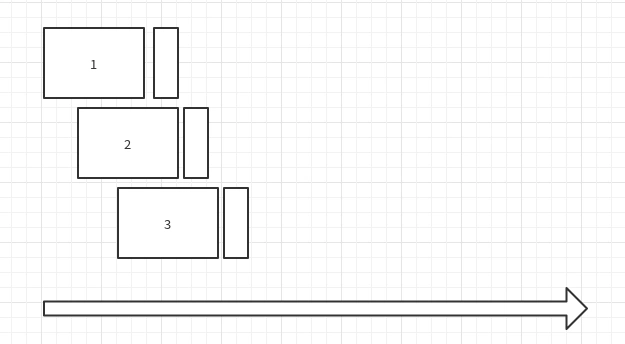
\includegraphics[height=4cm]{time_window.png}
	\caption{将所有数据按照时间窗口切分}
\end{figure}

我们需要先对 201901\_201903.csv/201910\_11.csv/20191201\_20191220.csv 中的数据进行预处理, 得到processed\_train\_data, 对
toPredict\_train\_gps.csv预处理得到processed\_test\_data. 利用processed\_train\_data和train\_TTI.csv中的数据可以训练模型, 由于需要
用前1小时的数据对后10-30分钟进行预测, 因此我们选择将所有数据按照时间窗口切分,分为训练集和验证集,并训练时间序列模型. 

在数据预处理的部分, 基本想法是遍历训练集, 根据网约车gps的信息、运动方向和各路口的位置统计出各
时间段经过各路口的车辆数. 由于训练集中已有路过车辆的平均速度, 因此暂时不考虑统计网约车的速度
情况. 由于路段具有一定长度, 并且不是一条直的线段, 所以我们用平行四边形近似表示路段区域, 将网
约车GPS看作一个点的坐标, 用点是否在区域中判断车辆是否经过这一路段. 再通过比较网约车的方向和路
段整体走向, 得出网约车具体经过哪一个方向的路段. 网约车gps数据清理的代码在 /data\_processing 中
经过数据预处理, 得出每个路口在各个时刻的车流量、TTI和通过路口的平均车速, 存入train\_\#name.csv中. 

在特征工程的部分, 基本思路是使用前60分钟的数据预测后30分钟的数据, 即用前60分钟的数据构成一个
24维的向量, 预测出一个三维向量. 这里的TimeSlice是当天的第$i$个10分钟. 获取输入和输出向量的
方法如下:
$$
\begin{aligned}
  x_i \leftarrow [&Speed1, Car1, TTI1, TimeSlice1, Speed2, Car2, TTI2, TimeSlice2,\\
  &Speed3, Car3, TTI3, TimeSlice3, Speed4, Car4, TTI4, TimeSlice4,\\
  &Speed5, Car5, TTI5, TimeSlice5, Speed6, Car6, TTI6, TimeSlice6]\\
	y_i \leftarrow [&TTI7,TTI8,TTI9],\ x_i \in \mathbb{R}^{24},\ y_i \in \mathbb{R}^3
\end{aligned}
$$

我们希望训练出一个h:
$$h:\mathbb{R}^{24} \rightarrow \mathbb{R}^3$$

基于mae误差, 求解以下优化问题:
$$\min _{h}\dfrac{1}{|D|}\left[\sum_{x_{i} \in D_x}\sum_{j=1}^3 | y_{ij}-h(x_i)_j | \right]$$

\section{基本理论和方法}
集成学习通过构建并结合多个学习器来完成学习任务. 根据集成学习“好而不同”的原理, 
使用随机森林、XGBoost、LightGBM作为个体学习器, 将他们进行结合, 以获得比单一学
习器更好的泛化能力. 集成学习主要有两种方法:boosting和bagging. boosting算法
的主要思想是首先根据初始训练集训练出一个基学习器, 然后根据基学习器的表现调整样本
权重, 使得基学习器预测较差的样本在后续受到更多关注, 重复这个过程, 直到基学习器
数量到达预先设定的T为止. bagging算法的主要思想是采用自主采样的方法从训练集中采
样得到T个样本集合, 使用每个采样集训练出一个学习器, 然后把这T个学习器的结果相结合. 

随机森林是一种bagging的方法, 它和传统bagging的区别在于它又引入了一种随机性——
属性选择的随机性. 随机森林算法对于决策树的每个节点, 先从该节点的属性集合种随机
选择包含k个属性的子集, 然后从中选出最优属性用于划分. 

XGBoost是一种boosting方法, 在梯度增强框架下实现机器学习算法. XGBoost提供了
一种并行的boosting算法(也称为GBDT、GBM), 可以快速、准确地解决许多数据科学问题. 

LightGBM基于XGBoost算法, 再引入一种随机性:保留梯度大于阈值的向量, 但是随机保
留梯度小于阈值的向量. Ke\cite{ref3}通过理论分析和实验证明这种随机性的引入可以使得结果优
于随机采样. 

\section{方法}
在数据预处理、特征工程(细节见Sec. 3 模型)之后, 为了便于后期处理, 我们对每个路
口进行了训练集和测试集的划分, 使得该问题转变为了一个典型的回归问题. 我们使用了开
源机器学习包sklearn、lightGBM、XGBoost、pytorch来完成回归任务. 

首先, 我们使用random forest这一传统的集成学习方法. 在gen\_train和gen\_test函数
中, 将输入的24维向量堆叠, 对每一个路口构成$2872 \times 24$维矩阵, 将输出的3维
向量堆叠, 构成$2872 \times 3$矩阵, 同理构成$84 \times 24$维测试输入矩阵. 使用
train\_test\_split划分训练集和验证集, 用$718 \times 24$的矩阵作为验证集输入,
$2154 \times 24$作为训练集输入. 随机森林参数使用默认参数, 调用
RandomForestRegressor的fit函数, 进行训练. 训练结束之后, 在验证集上计算l1误差. 
对于每一个路口调用RandomForestRegressor的predict函数进行预测. 

其次, 我们使用XGBoost这种典型的boosting方法. 依然是利用gen\_train和gen\_test函数
整理出输入向量,用train\_test\_split划分训练集和验证集. 输入向量$X$维度为$2872\time 24$,
$y$维度为$2872\times 3$, 随机划分比例为3:1. 训练模型时, 树的最大深度为6, 学习率为0.1, 
最小子权重为5, 生成的最大树的数目为150, 对于每棵树随机采样的比例为0.8, 防止过拟合, 设置
早停条件为验证集上10轮没有改善即停. 调用XBGRegressor中的fit函数进行训练, 并用predict
函数进行预测.

同时我们也使用了PCA降维之后的20维向量作为输入, 训练xgboost模型. 

然后, 我们使用lightGBM算法. 和前文相同, 进行训练集、验证集、测试集划分. 但是这里
有一点值得注意:lightGBM只支持预测实数值. 所以我们训练出3个模型分别用来预测后面的
三个时段, 最后将这三个结果拼接成一个向量. 在参数params设定中, 经过多轮实验和参数
调优, 最终我们设置参数中目标函数为l1 regression, 评估函数为l1 for regression,
学习率为0.1, 设置提升类型为gbdt, 最大迭代轮数为50轮, 早停条件为验证集上5轮没有
改善. 设置了早停的条件可以有效避免过拟合的问题. 调用lightgbm中的train函数进行训练,
最后使用lightgbm中的predict进行预测. 

最后, 我们通过将四种模型的预测结果加权融合, 得到最终预测结果. 

\section{方法分析}
我们比较了不同算法性能、收敛速度、稳定性、适用性四方面. 对于性能, 我们用训练耗费的时
间(单位秒)度量;对于收敛速度, 我们用训练耗费的迭代轮数来度量; 对于稳定性, 我们用5次
不同训练验证集划分下的mae的方差来度量;对于适用性, 在TTI预测问题中, 这两种模型都适
用, 所以我们设其为1. 绘制出雷达图如图2:

可以看出lightgbm的训练速度快于XGBoost, 这和Ke\cite{ref3}论文中提出来的论证结果是一致的, 
也体现了lightgbm在面对大量训练数据、高维特征的优越性, 尽管这个问题的数据量比较大, 
但是lightgbm通过GOSS的加入, 大大提高了运行速度. 

在迭代轮数方面, 两者相差很少. 

在稳定性方面, 实验次数不是很多, 初步体现出xgboost优于lightGBM, 但这一点还有待更多
实验. 

\begin{figure}[!htbp]
	\centering
	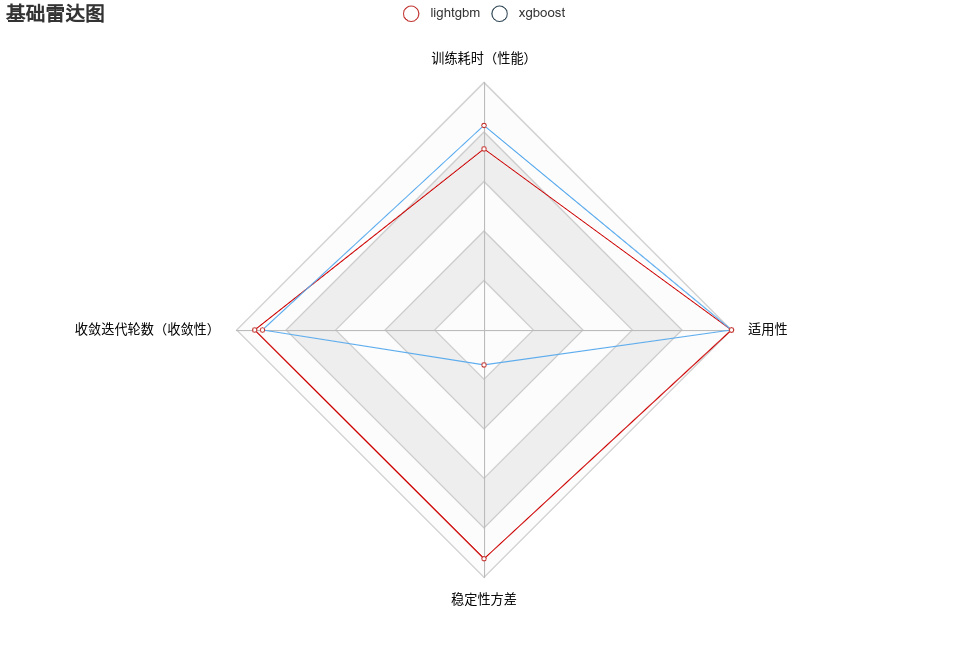
\includegraphics[height=4cm]{rader}
	\caption{不同算法性能、收敛速度、稳定性、适用性}
\end{figure}

\section{算法}
随机森林:
\begin{algorithm}[H]
  \caption{Random Forest}
  \begin{algorithmic}
      \STATE Input: Training set S , Features F and the number of trees in forest B
      \STATE function RandomForest(S,F)
        \STATE $H \leftarrow \emptyset$
        \FOR{$i \in 1,...,B$}
          \STATE $S^{(i)} \leftarrow A \  bootstrap \ sample \  from \ S$
          \STATE $h_i \leftarrow RandomizedTreeLearn(S^{(i)},F)$
          \STATE $H \leftarrow H \cup {h_i}$
        \ENDFOR
        \RETURN H
      \STATE function RandomizedTreeLearn(S,F)
        \FORALL{node}
          \STATE $f \leftarrow very \ samll \ subset \ of \ F$
          \STATE split on best feature in f
        \ENDFOR
      \RETURN learned tree   
  \end{algorithmic}
\end{algorithm}

XGBoost:
\begin{algorithm}[H]
  \caption{Exact Greedy Algorithm for Split Finding}
  \begin{algorithmic}
    \STATE Input: $I$ : instance set of current node
    \STATE Input: $d$ : feature dimension
    \STATE gain $\leftarrow 0$, $G \leftarrow \sum_{i\in I}g_i$, $H \leftarrow \sum_{i\in I}h_i$
      \FOR{$k \in 1,...,m$}
        \STATE $G_L \leftarrow 0, H_L\leftarrow 0$
        \FOR{$j \in $sorted(I, by $x_{jk}$)}
          \STATE $G_L \leftarrow G_L+g_j, H_L\leftarrow H_L+h_j$
          \STATE $G_R \leftarrow G-G_L, H_R\leftarrow H-H_L$
          \STATE score $\leftarrow max(score, \frac{G_L^2}{H_L+\lambda}+\frac{G_R^2}{H_R+\lambda}-\frac{G^2}{H+\lambda})$
        \ENDFOR
      \ENDFOR
  \end{algorithmic}
\end{algorithm}

近似搜索算法: 当数据太多不能装载到内存时, 不能进行精确搜索分裂, 只能近似. 
根据特征分布的百分位数, 提出特征的一些候选分裂点, 
将连续特征值映射到桶里(候选点对应的分裂), 然后根据桶里
样本的统计量, 从这些候选中选择最佳分裂点.
\begin{algorithm}[H]
  \caption{Approximate Algorithm for Split Finding}
  \begin{algorithmic}
    \FOR{$k \in 1,...,m$}
      \STATE Propose $S_k=\{s_{k1}, s_{k2},...,s_{kl}\}$ by precentiles on feature k.
      \STATE Proposal can be done per tree (global), or per split (local).
    \ENDFOR
    \FOR{$k \in 1,...,m$}
        \STATE $G_{kv} \leftarrow=\sum_{j\in\{j|s_{k,v}\geq x_{jk}\geq s_{k,v-1}\}}g_j$
        \STATE $H_{kv} \leftarrow=\sum_{j\in\{j|s_{k,v}\geq x_{jk}\geq s_{k,v-1}\}}h_j$
    \ENDFOR
    \STATE Follow same step as in previous sectio to find max
    \STATE score only among proposed splits.
  \end{algorithmic}
\end{algorithm}

LightGBM:
\begin{algorithm}[H]
  \caption{Gradient-based One-Side Sampling}
  \begin{algorithmic}
    \STATE Input: $I$ : training data, $d$ : iterations
    \STATE Input: $a$ : sampling ratio of large gradient data
    \STATE Input: $b$ : sampling ratio of small gradient data
    \STATE Input: $loss$ : loss function, $L$ : weak learner
    \STATE models $\leftarrow \{\}$, fact $\leftarrow \frac{1-a}{b}$
    \STATE topN $\leftarrow $ a $\times$ len(I), \ randN $\leftarrow$ b $\times$ len(I)
      \FOR{$i \in 1,...,d$}
        \STATE preds $\leftarrow$ models.predict($I$)
        \STATE g $\leftarrow$ $loss$($I$,preds), w $\leftarrow$ {1,1,...}
        \STATE sorted $\leftarrow$ GetSortedIndices(abs(g))
        \STATE topSet $\leftarrow$ sorted[1:topN]
        \STATE randSet $\leftarrow$ RandomPick(sorted[topN:len(I)],randN)
        \STATE usedSet $\leftarrow$ topSet + randSet
        \STATE w[randSet] $\times = $ fact $\rhd$ Assign  weight $fact$  to the small gradient data
        \STATE newModel $\leftarrow$ L($I$[usedSet],-g[usedSet],w[usedSet])
        \STATE models.append(newModel)
      \ENDFOR
  \end{algorithmic}
\end{algorithm}
  
\begin{algorithm}[H]
  \caption{Merge Exclusive Features}
  \begin{algorithmic}
    \STATE Input: $numData$ : number of data
    \STATE Input: $F$ : One bundle of exclusive features
    \STATE Output: newBin, binRanges
    \STATE binRanges $\leftarrow \{0\}$, totalBin $\leftarrow 0$
      \FOR{$f \in 1,...,F$}
        \STATE totalBin += f.numBins
        \STATE binRanges.append(totalBin)
      \ENDFOR
        \STATE newBin $\leftarrow$ new Bin(numData) 
      \FOR{$i \in 1,...,numData$}
        \STATE newBin[i] $\leftarrow$ 0
        \FOR{$j \in 1,...,len(F)$}
          \IF{$F[j].bin[i] \neq 0$}
            \STATE newin[i] $\leftarrow$ F[j].bin[i] + binRanges[j]
          \ENDIF
        \ENDFOR
      \ENDFOR
  \end{algorithmic}
\end{algorithm}

模型融合:
\begin{algorithm}[H]
	\caption{Final}
	  \begin{algorithmic}  %1表示每隔一行编号	
      \STATE Input: x$\in \mathbb{R}^{m\times 24}$, y$\in \mathbb{R}^{m\times 3}$, x\_test$\in \mathbb{R}^{n\times 24}$
      \STATE Output:  y\_test$\in \mathbb{R}^{n\times 3}$
        \STATE x\_PCA = PCA(x), x\_PCA\_test = PCA(x\_test)
        \STATE x\_PCA\_train, x\_PCA\_valid, y\_PCA\_train, y\_PCA\_valid = split(x\_PCA, y)
        \STATE x\_train, x\_valid, y\_train, y\_valid = split(x, y)
        \STATE validset = (x\_valid, y\_valid)
        \STATE validPCAset = (x\_PCA\_valid, y\_PCA\_valid)
        \STATE model1 = xgboost.train(x\_train, y\_train, validset)
        \STATE model2 = lightgbm.train(x\_train, y\_train, validset)
        \STATE model3 = random\_forest.train(x\_train, y\_train, validPCAset)
        \STATE model4 = xgboost.train(x\_PCA\_train, y\_PCA\_train)
        \STATE pred1 = model1.predict(x\_test)
        \STATE pred2 = model2.predict(x\_test)
        \STATE pred3 = model3.predict(x\_test)
        \STATE pred4 = model4.predict(x\_PCA\_test)
	    \RETURN 0.405 * pred1 + 0.45 * pred2 + 0.1 * pred3 + 0.045 * pred4
	  \end{algorithmic}
  \end{algorithm}

\newpage
\section{算法分析}
由于我们的具体问题是一个工程性的回归预测问题, 所以算法分析部分不是本次报告的重点. 下面我们简要的论述一下各个算法的时间复杂度分析结果.

\begin{enumerate}
  \item 首先是random forest的算法分析. 根据Louppe\cite{ref4}的分析, 随机森林的时间复杂度可以概括为(表格里面不好打公式, 公式在图片里), 这里M是基学习器数量, N表示样本数, K表示每个节点随机选择的属性数量, $\bar{N}$表示0.632*N.
  \item 其次是XGBoost, 其目标函数定义为: 
  $$\mathcal{L}=\sum_{i=1}^nl(y_i,\hat{y}_i)+\sum_{k=1}^K\Omega(f_k)$$
  目标函数由两部分组成, $\sum_{i=1}^nl(y_i,\hat{y}_i)$用于衡量预测值与真实值的差距, $\sum_{k=1}^K\Omega(f_k)$则是正则化项. 正则化项同样包含两部分, $\Omega(f)=\gamma T+\dfrac{1}{2}\lambda\|\omega\|^2$. $T$表示叶子结点的个数, $\omega$表示叶子节点的分数, $\gamma$可以控制叶子结点的个数, $\lambda$可以制叶子节点的分数不会过大, 防止过拟合.
  
  生成$t$棵树后, 预测分数可以写成$\hat{y}_i^{(t)}=\hat{y}_i^{(t-1)}+f_t(x_i)$. 代入目标函数后在$f_t=0$处泰勒展开, 去掉前$t$棵树的预测分数与​的残差(对目标函数不影响), 简化目标函数为:
  $$\mathcal{L}^{(t)}=\sum_{i=1}^n\left[g_if_t(x_i)+\dfrac{1}{2}h_if_t^2(x_i)\right]+\Omega(f_t)$$
  其中$g_i=\partial_{\hat{y}^{(t-1)}}l(y_i,\hat{y}^{(t-1)})$, $h_i=\partial^2_{\hat{y}^{(t-1)}}l(y_i,\hat{y}^{(t-1)})$, 为一阶和二阶梯度.
  
  上式是将每个样本的损失函数值加起来, 而每个样本都最终会落到一个叶子结点中, 所以我们可以将所以同一个叶子结点的样本重组起来, 得到:
  $$\mathcal{L}^{(t)}=\sum_{j=1}^{T}\left[\left(\sum_{i\in I_j}g_i\right)\omega_j+\dfrac{1}{2}\left(\sum_{i\in I_j}h_i+\lambda\right)\omega_j^2\right]+\gamma T$$
  通过上式的改写, 可以将目标函数改写成关于叶子结点分数$\omega$的一个一元二次函数, 求解最优的​和目标函数值就变得很简单了.
  \item 最后是lightGBM. 这种算法是在XGBoost的基础上进行改进, 加入了GOSS和EFB算法, 从而大大提高了速度. 所以我们这里简要分析一下为什么加入它们之后可以大大提高速度. 首先是GOSS, GOSS通过随机去除一些梯度小于阈值的样本, 起到了减少训练样本的作用, 可以一定程度地提高训练速度. 同时, Ke【引用编号】在论文中通过定理3.2的分析
  $$\epsilon (d) \leq C_{a,b}^2 \ln \frac{1}{\delta} \cdot \max\{ \frac{1}{n_{l}^{j}(d) },\frac{1}{n_{r}^{j}(d)}\}+2DC_{a,b}\sqrt{ \frac{\ln{\frac{1}{\delta}}}{n}}$$
  得到误差项取决于
  $$\sqrt{\frac{1}{n}}$$
  所以, 当$n \rightarrow \infty$, 该误差
  $$\epsilon \rightarrow 0$$
  即两者误差很小. 所以GOSS方法达到了在几乎不损失精度的情况下, 加快了训练速度的效果. 
  
  如果两个特征是互斥的, 那么可以将两个特征合为一个特征. EFB就利用了这个原理. 加入EFB将原训练集中稀疏而且互斥的特征变成一个特征, 减少了特征数量, 
  $$O(data \times feature)$$
  转变为
  $$O(data \times bundle)$$
  可以加快训练速度.
\end{enumerate}

各算法时间复杂度对比: 
\begin{table}[!htbp]
  \centering
  \begin{tabular}{|c|c|c|c|}
    \hline
    算法 & 最好情况 & 最坏情况 & 平均情况\\
    \hline
    CART&$\Theta(pN\log^2N)$&$O(pN^2\log N)$&$\Theta(pN\log^2N)$\\
    \hline
    Bagging&$\Theta(Mp\tilde{N}\log^2\tilde{N})$&$O(Mp\tilde{N}^2\log\tilde{N})$&$\Theta(Mp\tilde{N}\log^2\tilde{N})$\\
    \hline
    随机森林&$\Theta(MK\tilde{N}\log^2\tilde{N})$&$O(MK\tilde{N}^2\log\tilde{N})$&$\Theta(MK\tilde{N}\log^2\tilde{N})$\\
    \hline
    ETs&$\Theta(MKN\log N)$&$\Theta(MKN^2)$&$\Theta(MKN\log N)$\\
    \hline
    PERT&$\Theta(MN\log N)$&$\Theta(MN^2)$&$\Theta(MN\log N)$\\
    \hline
  \end{tabular}
\end{table}

\section{数值结果}
实验环境: windows + Intel Core i5 + Python 3.7.6; Ubuntu 18.04.4 LTS + Intel Core i5 + Python 3.6.9
\begin{enumerate}
  \item 观察数据:利用部分网约车的GPS信息, 绘制其行车路线图:
  \begin{figure}[!htbp]
    \centering
    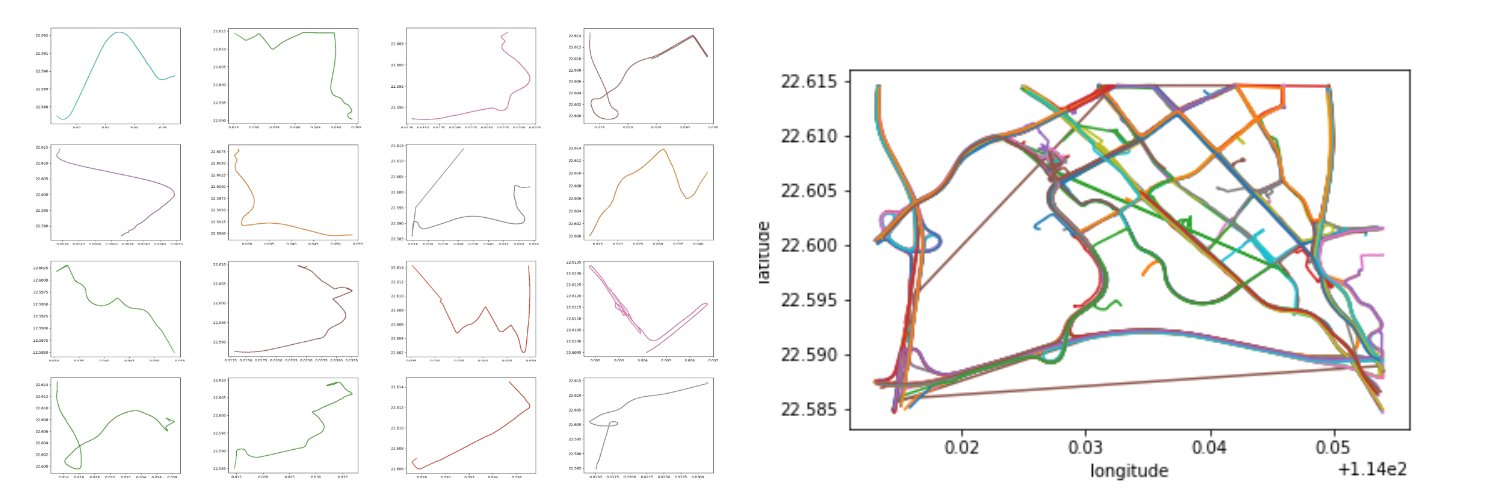
\includegraphics[height=3cm]{road_image.png}
    \caption{部分网约车行车路线图}
  \end{figure}
  \item 数据预处理:利用部分网约车的GPS和速度信息, 在地图上绘制拥堵状况热力图, 其中速度越小对应的数值越大, 即色温越高的地方越拥堵:
  \begin{figure}[!htbp]
    \centering
    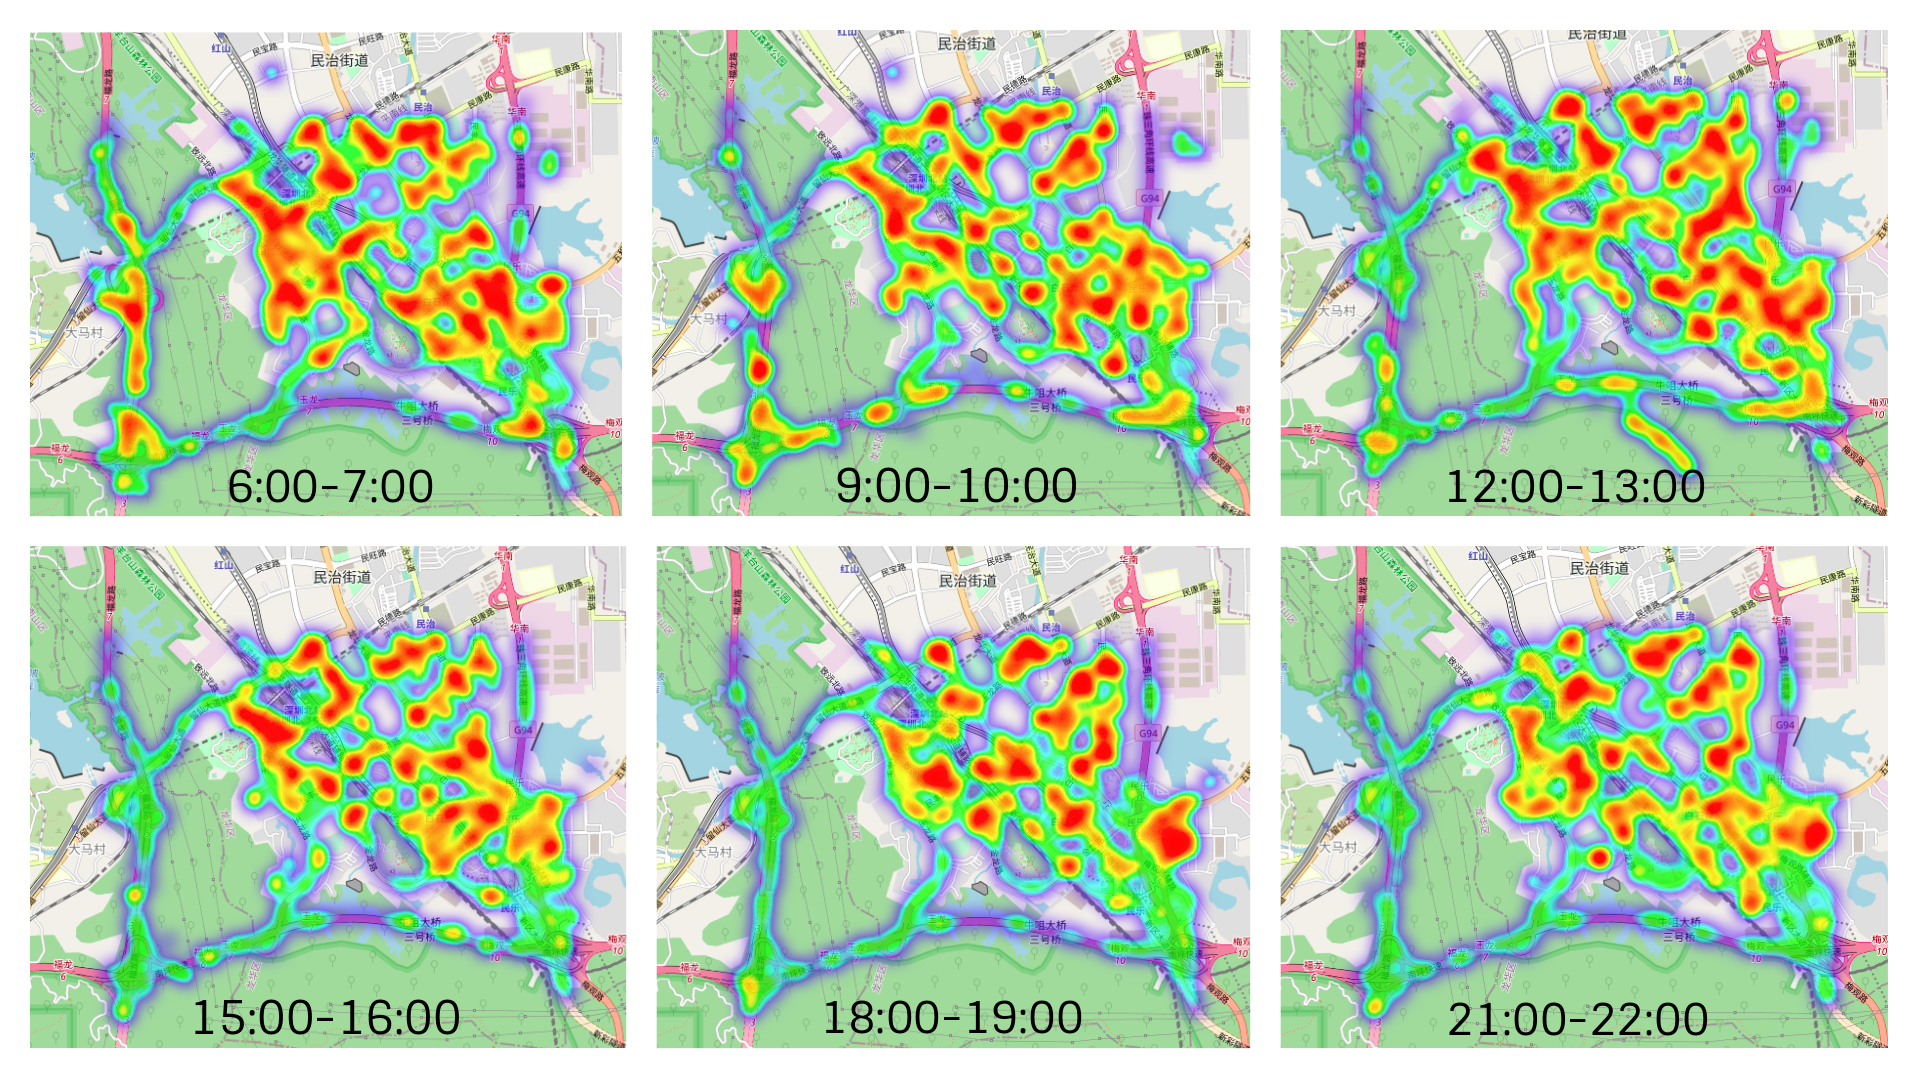
\includegraphics[height=3cm]{heatmap.png}
    \caption{拥堵状况热力图}
  \end{figure}
  \item 绘制了三个模型(lightgbm, xgboost, random\_forest)在各个路口验证集上的mae误差如下图:
    \begin{figure}[!htbp]
      \centering
      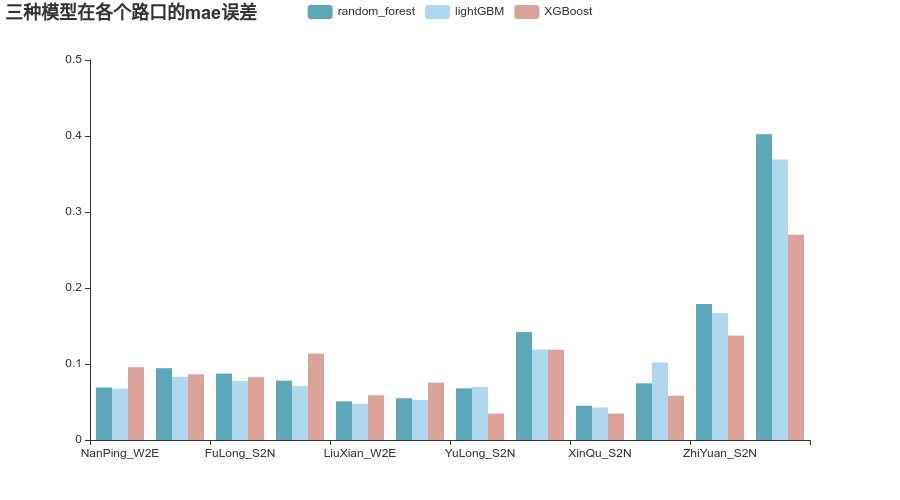
\includegraphics[height=4cm]{bar.png}
      \caption{模型在各个路口验证集上的mae误差}
    \end{figure}
\end{enumerate}

\section{讨论}
在讨论部分中, 我们主要研究了:
\begin{enumerate}
  \item 用XGBoost在验证集上进行测试, 发现用六个时间段预测之后的三个时间段, 尽管分别训练了三个模型, 但是效果仍是越来越差, 这是因为第三个时间段相较前两个与输入的六个时间段的相关性变小了, 效果自然不如之前的:
      \begin{figure}[!htbp]
        \centering
        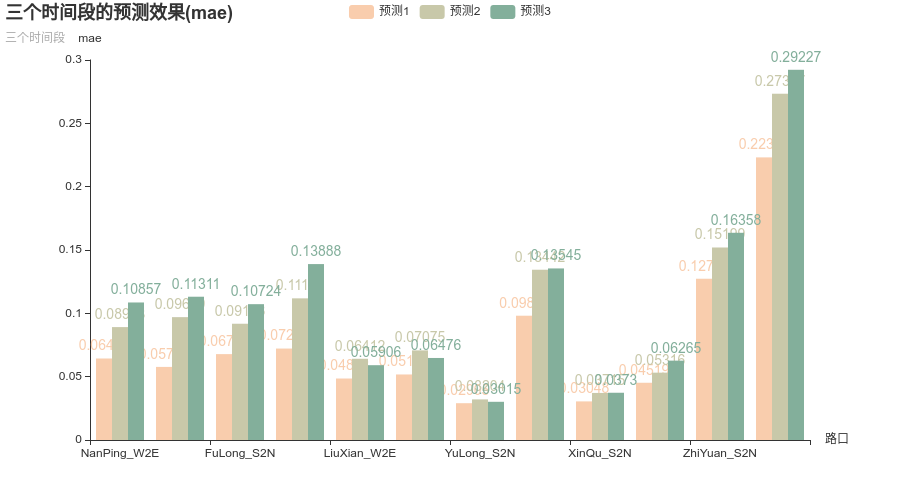
\includegraphics[height=4cm]{bar2.png}
        \caption{验证集上三个时间段的预测效果}
      \end{figure}
  \item 在TTI回归问题中降维、聚类、继承有效性的问题. 首先是KMeans聚类. 最初我们根据交通拥堵指数问题实际情况, 考虑TTI可能会在不同时间段有不同分布模型, 所以我们对输入的向量先进行了聚类, 然后在 每一类中进行回归预测. 但是, 效果并不理想, 最终我们放弃了先进行聚类的想法. 实验结果见下表格. 我们希望找到该问题不适合采用Kmeans聚类的原因. 
      \begin{table}[!htbp]
      \centering
        \begin{tabular}{|c|c|}
          \hline
          簇数 & 验证集误差\\
          \hline
          1 & 0.118500\\
          \hline
          2 & 0.147335\\
          \hline
          3 & 0.121700\\
          \hline
          5 & 0.131066\\
          \hline
        \end{tabular}
      \end{table}

      然后我们考虑使用降维进行数据可视化, 我们对回归问题中每一个路口输入的24维向量进行PCA
      降维, 降到2维, 然后以此作为x,y轴, 绘制出图像如图7. 
      
      容易看出, 在每个路口的图像中, 图形都近似团成一簇, 只有少量点散落在簇外, 直观上并没有多簇的情况. 再结合kmeans
      的原理, 我们认为kmeans会把原先的一团分成几部分, 反而破坏了模型的泛化能力, 所以导致
      加入聚类效果不佳. 同时由于降维之后我们发现有很少的点散落在簇外, 我们考虑了异常点的情况. 由于PCA降维有利有弊, 既可以通过取较大的特征值对应的特征向量来去除噪音, 也会丢失一部分特征信息, 所以我们用降维前后的数据分别训练2种xgboost模型, 然后根据问题实际特点将它们的预测结果加权相加, 我们希望通过这种方法能够尽可能保留有效特征又去除一些噪音影响. 

      最后, 我们根据各个模型在各路口预测结果的mae误差图(图5), 可以看出这三个模型在不同路口总体表现相似, 
      但是在不同路口三种模型各有优劣. 所以, 我们希望按照不同权重将它们结合起来, 以得到更
      高的泛化能力. 经过实验, 最终确定权重见伪代码. 通过这一步, 可以将泛化误差从0.1144降低到0.1070.

      \begin{figure}[htbp]
        \centering
        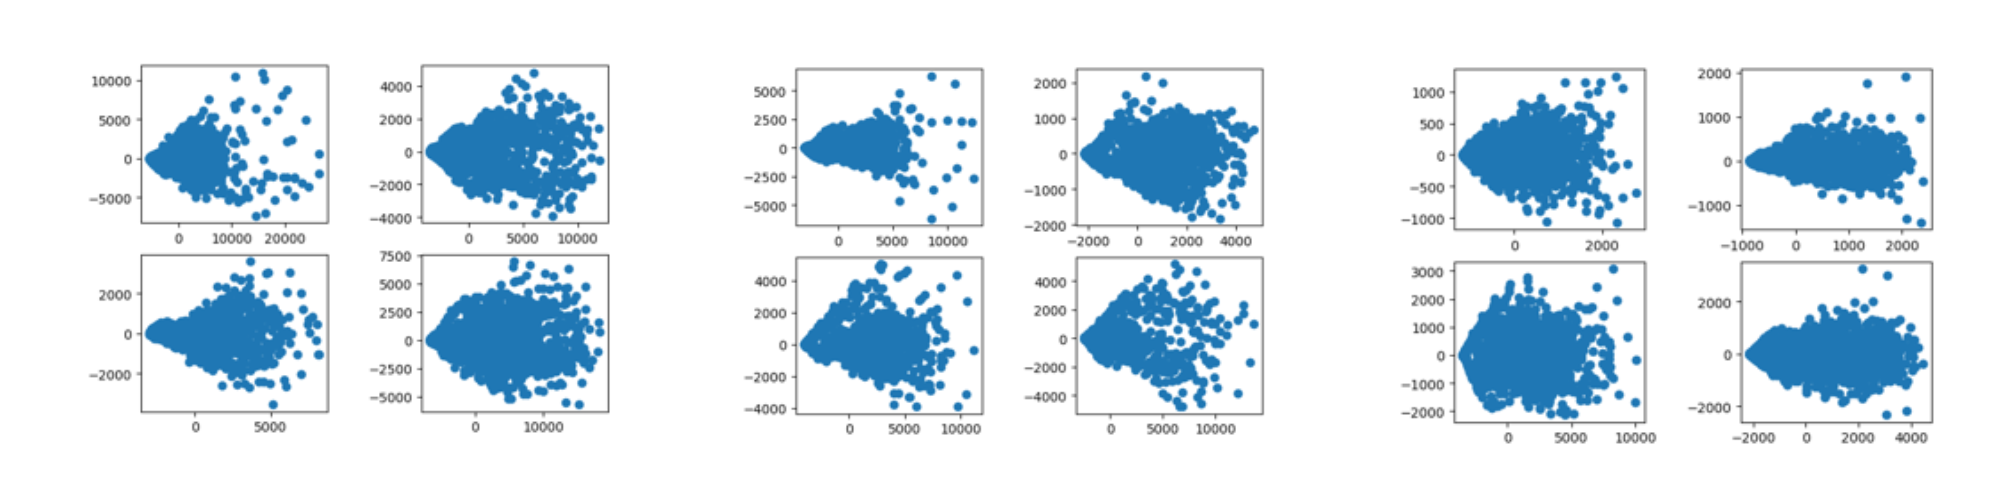
\includegraphics[height=4cm]{PCA.png}
        \caption{PCA}
      \end{figure}

  \end{enumerate}
\section{结论}
经过实验, 我们得到以下结论:
\begin{enumerate}
  \item 尽管针对每个路口的每个样本, 针对三个时间段训练了不同的模型, 
  但预测效果是model1 > model2 > model3.
  \item 集成学习的效果要好于单一模型, 这体现在实验过程中, 吕志存曾
  尝试用lstm进行预测, 但效果比随机森林和XGBoost差很多.
  \item 将多个模型预测的结果取加权和会比随机森林(RF)、XBGoost、LightGBM、XGBoost+PCA
  效果更好. 最终确定的权值为:0.405*xgb+0.45*(xgb+PCA)+0.1*RF+0.045*lightgbm. 
  在测试集上得到了最好的结果0.1070.
  \item 此外我们还有一些想法, 因为时间限制暂时没能着手实践:
    \begin{itemize}
      \item 我们整理出的每个样本可以表示为(f1, f2, f3, f4, f5, f6)->(t7, t8, t9), 
      其中1~9代表了时间顺序, 在本实验中, 我们根据前6个特征, 直接用三个模型分别对后三个TTI
      进行预测, 我们更希望能用第一个模型的预测结果加入到第二个模型的输入中去, 将第二个模型的
      预测结果加入到第三个模型的输入中去. 这样也许能得到更好的结果. 
      \item 我们发现致远路的预测效果很差, 我们希望针对致远路单独进行调试, 也许能得到更好的结果. 
      \item 我们发现被融合的4个模型在12个路口的表现各不相同, 我们希望能针对12个路口分别调整4个
      模型的权值, 也许能得到更好的结果. 
    \end{itemize}
\end{enumerate}

\section{致谢}
感谢助教老师提供了针对数据竞赛的阅读材料和撰写论文的建议.

感谢为我们提供了优秀的开源模型的团队们.

\section{参考文献}
\bibliographystyle{plain}
\bibliography{ref.bib}

\section{组员贡献}
\begin{itemize}
	\item 181220067 张含笑: GPS轨迹绘制和观察,部分数据清洗,数据集划分,XGBoost回归,报告部分内容撰写
	\item 181220038 吕志存: 部分数据清洗,RF回归,LightGBM回归,集成学习参数调整,报告部分内容撰写
\end{itemize}

\section{附录}
我们使用git来管理代码,github项目地址: \url{https://github.com/Michelia-zhx/Huaweicloud_Competition_Traffic}

\renewcommand*\DTstylecomment{\rmfamily\color{blue}} \renewcommand*\DTstyle{\ttfamily}
\dirtree{%
  .1 /.
  .2 algorithm\DTcomment{不同算法的应用于本次TTI预测问题的代码}.
  .3 train\_array\DTcomment{读入训练集的中间结果}.
  .3 gen\_train\_npy.py\DTcomment{产生中间结果,暂时存到train\_array中}.
  .3 lightgbm.py\DTcomment{使用lightGBM处理回归问题}.
  .4 train(train\_df, test\_df, params)\DTcomment{使用lightgbm进行训练}.
  .4 predict(road\_id, timestamp, train\_TTI, test\_gps, models)\DTcomment{使用\\训练出的lightgbm模型进行预测}.
  .3 lstm.py\DTcomment{使用LSTM模型处理回归问题}.
  .3 random\_forest2.py\DTcomment{使用随机森林处理回归问题}.
  .4 train(df,rf1)\DTcomment{使用随机森林在训练集上训练}.
  .4 predict(road\_id, timestamp, train\_TTI, test\_gps, lst)\DTcomment{利用lst中的模型对road\_id在timestamp时的TTI进行预测}.
  .3 with\_cluster\_xgboost\_alg.py.
  .4 gen\_train()\DTcomment{把数据经过特征工程变为24维的输入向量}.
  .4 gen\_test()\DTcomment{把测试数据经过特征工程变为24维的输入向量}.
  .4 train()\DTcomment{训练模型}.
  .4 evaluate()\DTcomment{使用model在X上进行评价}.
  .4 predict()\DTcomment{使用model对测试集进行预测}.
  .3 xgboost\_alg.py\DTcomment{使用XGBoost处理回归问题}.
  .4 train(train\_X, train\_y, eval\_X, eval\_y, road\_index)\DTcomment{对r训练集oad\_index路口,train\_X,train\_y作为, eval\_X, eval\_y作为验证集,进行训练}.
  .4 gen\_test(model, pred\_df)\DTcomment{进行特征工程,并对测试集产生预测结果}.
  .4 evaluate(model, X, y)\DTcomment{评价model在X上的mae误差}.
  .2 data\_preprocessing\DTcomment{数据预处理的代码}.
  .3 count\_car.py\DTcomment{通过对每10分钟经过\\各个路口的网约车计数,得到以十分钟为粒度的车流量数据}.
  .3 gen\_testset.py\DTcomment{产生每个路口的测试集}.
  .3 gen\_trainset.py\DTcomment{产生每个路口的训练集}.
  .2 datasets\DTcomment{将训练数据和测试数据按照路口划分之后保存的csv结果}.
  .2 photo\DTcomment{根据20191201-20191220.csv中部分网约车的GPS信息,绘制出的GPS图形}.
  .3 draw\_road.py\DTcomment{绘制出20191201-20191220.csv中\\一部分网约车GPS图形,以经度作为横轴,维度作为纵轴}.
  .2 processed\_test\_data\DTcomment{根据测试集上网约车GPS\\整理出的各个10分钟内每个路口的车流量}.
  .2 processed\_train\_data\DTcomment{根据训练集上网约车GPS\\整理出的各个时刻每个路口的车流量}.
  .2 traffic\DTcomment{部分训练集和测试集数据}.
  .2 README.md\DTcomment{项目背景和题目要求}.
}

\end{document}